\documentclass{article}
\usepackage{graphicx}
\usepackage{amssymb}
\usepackage{fixltx2e}
\usepackage{amsmath}
\usepackage{mathtools}
\usepackage{siunitx}
\usepackage[]{algorithm2e}

\title{Inverse Kinematics for Human Fingers \\ \large Report}
\date{2016/10/26}
\author{3858103 - Ricky van den Waardenburg}

\begin{document}
\maketitle
\newpage

\section{Introduction}

The finger that was assigned to me was the little finger. More details on the little finger can be found in the \textit{Mathematical model} section of this report. The end goal of this practical exercise is creating an inverse kinematics solver for a human finger. The inverse kinematics solver I have implemented is written using C++, OpenGL, SDL2.0 and the SDL2\_ttf library. \\\\The source code for my IK solver can be found on the repository on Github at \textit{https://github.com/Daimao/inverse-kinematics} and will be made public after the report is due.

\section{Mathematical model}

A basic analysis of the situation described by the practical exercise reveals that the model contains a finger consisting of three 1-DOF joints and 3 links (4 including the base link). All joints in this model rotate in the z-axis and are limited by a an angular constraint as described in the joint constraint table. Since joints rotate only around the z-axis, all movement happens in the \textit{(x,y)} plane. The links have lengths based on measurements and are found in the link length table below. The maximum range (added length of all links) is represented below as the blue circle and the unbound object \textit{O} is represented as the green line below the x-axis.

\begin{figure}[h!]
\centering
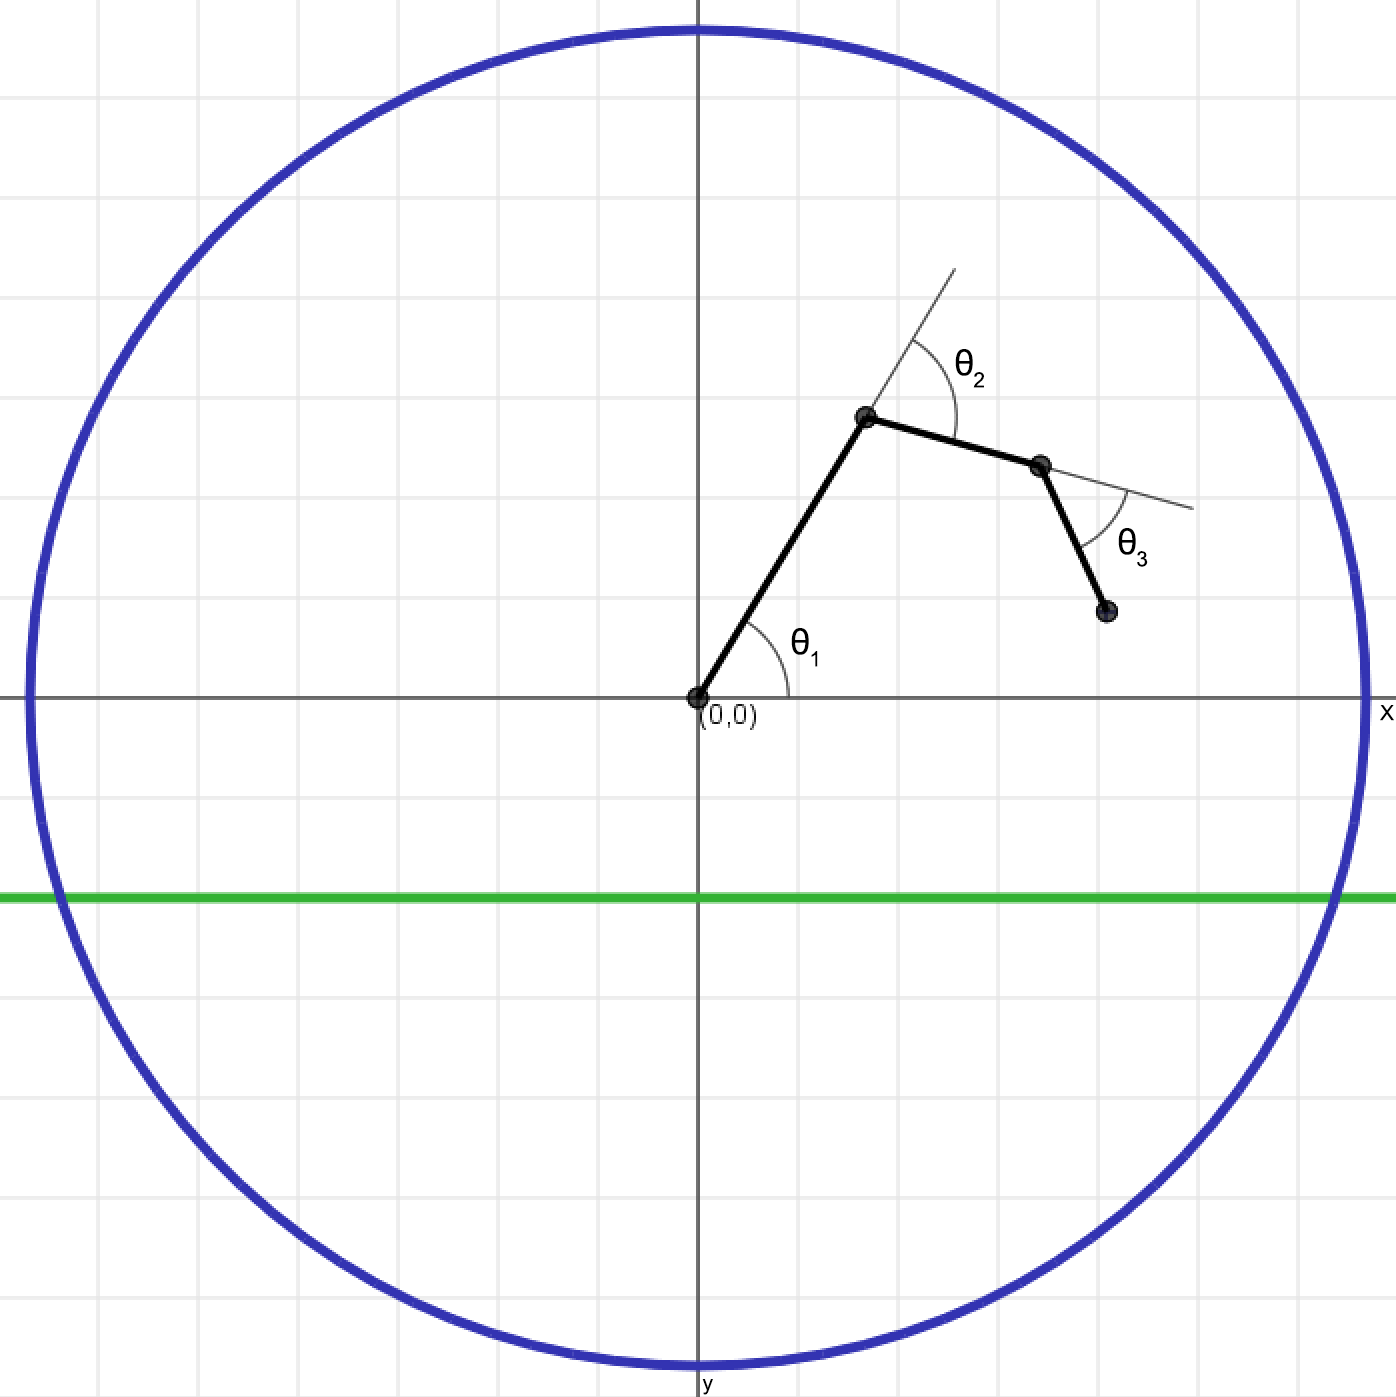
\includegraphics[scale=0.15]{situation.png}
\caption{Situation sketch.}
\end{figure}

\begin{table}[h!]
\centering
\caption{Link lengths}
\label{my-label}
\begin{tabular}{lll}
\hline
\textbf{Link}                 & \textbf{Length} (in mm) &  \\\hline
Proximal phalanx     & 32.7           &  \\
Intermediate phalanx & 18.1           &  \\
Distal phalanx       & 16.0           & \\\hline
\end{tabular}
\end{table}

\begin{table}[h!]
\centering
\caption{Joint constraints}
\label{my-label}
\begin{tabular}{llll}
\hline
\textbf{Joint}                 & \textbf{Min.} (in rad) & \textbf{Max.} (in rad) & \\\hline
Metacarpophalangeal joint & \(-\pi/3\) & \(\pi/3\)\\
Proximal interphalangeal joint  & \(-2\pi/3\) & 0\\
Distal interphalangeal joint  & \(-2\pi/3\) & 0\\\hline
\end{tabular}
\end{table}

\subsection{Forward kinematics}

To perform a forward kinematics analysis the Denavit-Hartenberg is used. The planar model described in the previous section has 3 1-DOF, revolute joints (\textit{n = 3}, so in total it will have 4 links (\textit{n = n + 1}). Numbering of links starts at (0) for the \textit{base link} and continues to (1) for the proximal phalanx, (2) for the intermediate phalanx and (3) for the distal phalanx. Numbering of joints starts from (1) for the metacarpophalangeal joint, (2) for the proximal interphalangeal joint and (3) for the distal interphalangeal joint.

\begin{figure}[h!]
\centering
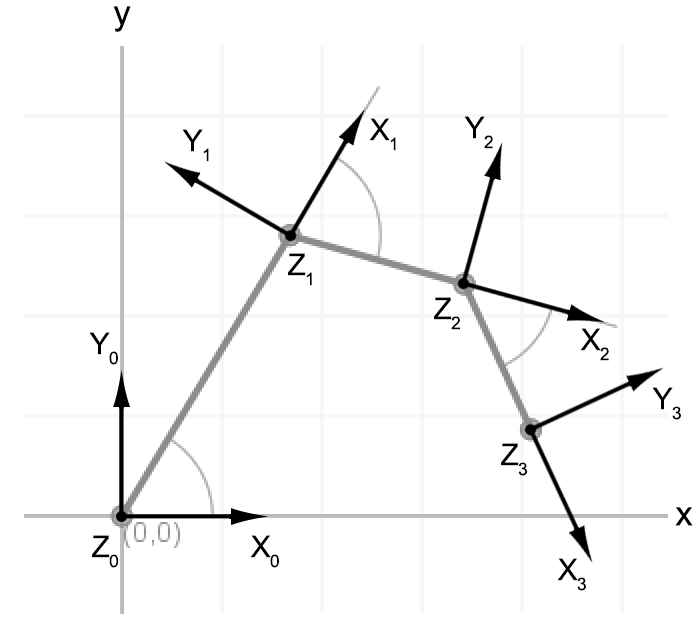
\includegraphics[scale=0.25]{situation3.png}
\caption{Coordinate frame assignment}
\end{figure}

A local coordinate frame Bi is assigned to each link (i) at joint i +1 using the Denavit-Hartenberg method. The result of which is visible in the coordinate frame assignment figure. The z-axes in this figure point out of the page and are drawn as a dot to prevent an unclear situation sketch. \\\textbf{Note:} the rule of aligning z to the direction of approach of the tool frame was skipped to keep the x- and y-axes in the same plane, as described by the practical exercise. The direction of approach is now out of the page, but for our implementation of the inverse kinematics solver this will not matter.  \\All axes needed for our transformation matrices are now present, only the link parameters are needed now. The link parameters were extracted from the data values presented earlier.

\begin{table}[h!]
\centering
\caption{Link parameters}
\label{my-label}
\begin{tabular}{lllll}
\hline
Frame No. & \(a_i\) & \(\alpha_i\) & \(d_i\) & \(\theta_i\) \\\hline
1 & 32.7 (PP) & 0      & 0  & \(\theta_1\) \\
2 & 18.1 (IP) & 0      & 0  & \(\theta_2\) \\
3 & 16.0 (DP) & 0      & 0  & \(\theta_3\) \\\hline
\end{tabular}
\end{table}

Since all joints are revolute joints, only \(\theta_1\),  \(\theta_2\) and \(\theta_3\) are variables, as such \(q = \begin{bmatrix}\theta_1\\\theta_2\\\theta_3\\\end{bmatrix}\). Using the link parameters we can create the transformation matrices for our forward kinematics equation.\\

\begin{figure}[h!]
\centering
\(T_1^0 = \begin{bmatrix}
       		\cos(\theta_1) & -\sin(\theta_1) & 0 & PP\cos(\theta_1) \\[0.3em]
       		\sin(\theta_1) & \cos(\theta_1) & 0 & PP\sin(\theta_1) \\[0.3em]
       		0 & 0 & 1 & 0 \\[0.3em]
       		0 & 0 & 0 & 1 \\[0.3em]
     \end{bmatrix}\)
\end{figure}

\begin{figure}[h!]
\centering
\(T_2^1 = \begin{bmatrix}
       		\cos(\theta_2) & -\sin(\theta_2) & 0 & IP\cos(\theta_2) \\[0.3em]
       		\sin(\theta_2) & \cos(\theta_2) & 0 & IP\sin(\theta_2) \\[0.3em]
       		0 & 0 & 1 & 0 \\[0.3em]
       		0 & 0 & 0 & 1 \\[0.3em]
     \end{bmatrix}\)
\end{figure}

\begin{figure}[h!]
\centering
\(T_3^2 = \begin{bmatrix}
       		\cos(\theta_3) & -\sin(\theta_3) & 0 & DP\cos(\theta_3) \\[0.3em]
       		\sin(\theta_3) & \cos(\theta_3) & 0 & DP\sin(\theta_3) \\[0.3em]
       		0 & 0 & 1 & 0 \\[0.3em]
       		0 & 0 & 0 & 1 \\[0.3em]
     \end{bmatrix}\)
\end{figure}

\begin{figure}[h!]
\centering
\(T_3^0 = T_1^0 * T_2^1 * T_3^2 = \begin{bsmallmatrix}
       		\cos(\theta_1+\theta_2+\theta_3) & -\sin(\theta_1+\theta_2+\theta_3) & 0 & PP\cos(\theta_1) + IP\cos(\theta_1 + \theta_2) + DP\cos(\theta_1 + \theta_2 +\theta_3) \\
       		\sin(\theta_1+\theta_2+\theta_3) & \cos(\theta_1+\theta_2+\theta_3) & 0 & PP\sin(\theta_1) + IP\sin(\theta_1 + \theta_2) + DP\sin(\theta_1 + \theta_2 +\theta_3) \\
       		0 & 0 & 1 & 0 \\
       		0 & 0 & 0 & 1 \\
     \end{bsmallmatrix}\)
\end{figure}

Using the transformation matrix \(T_3^0\) we can calculate the tip position, since coordinate frame 0 at (x,y,z)-coordinates (0,0,0) is regarded as world-space in the solver by multiplying with \(\begin{bmatrix}0&0&0&1\\\end{bmatrix}^T\).\\

Experimenting with different angular values gives us two different configurations with the same tip position at (x,y)-coordinates (3, -2).

\(q_{left} = \begin{bmatrix}-3.6\si{\degree}\\-40.8\si{\degree}\\-116\si{\degree}\\\end{bmatrix}, q_{right} = \begin{bmatrix}25.2\si{\degree}\\-114.6\si{\degree}\\0.0\si{\degree}\\\end{bmatrix}\)

\begin{figure}[h!]
\centering
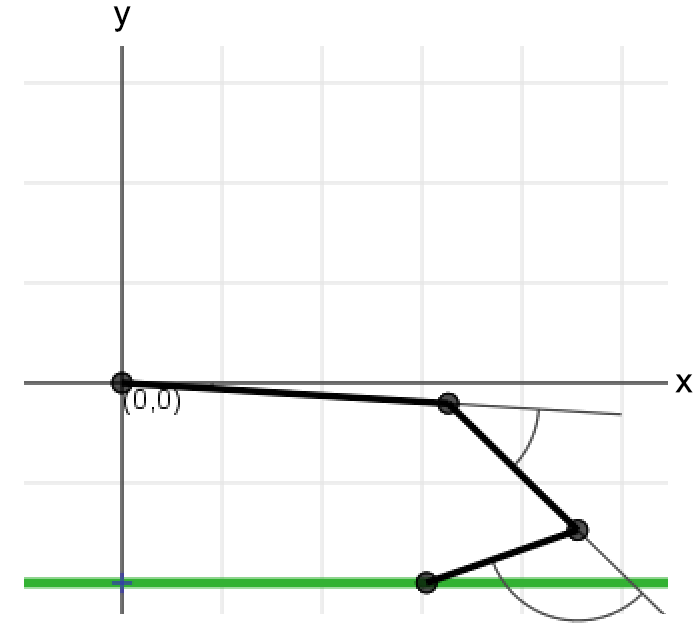
\includegraphics[scale=0.2]{substitute1.png}
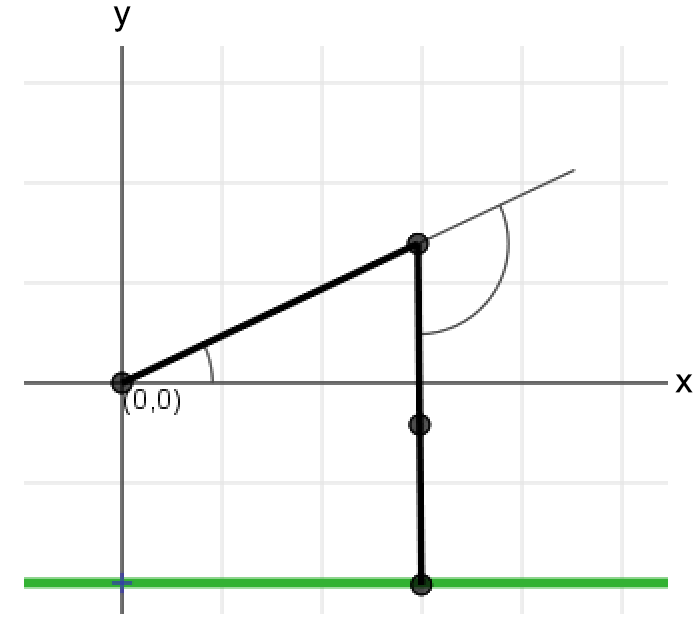
\includegraphics[scale=0.2]{substitute2.png}
\caption{Two configurations with different angular values}
\end{figure}

Experimenting with values between the angle variables' limits, an image of reachable positions was generated by the solver.

\begin{figure}[h]
\centering
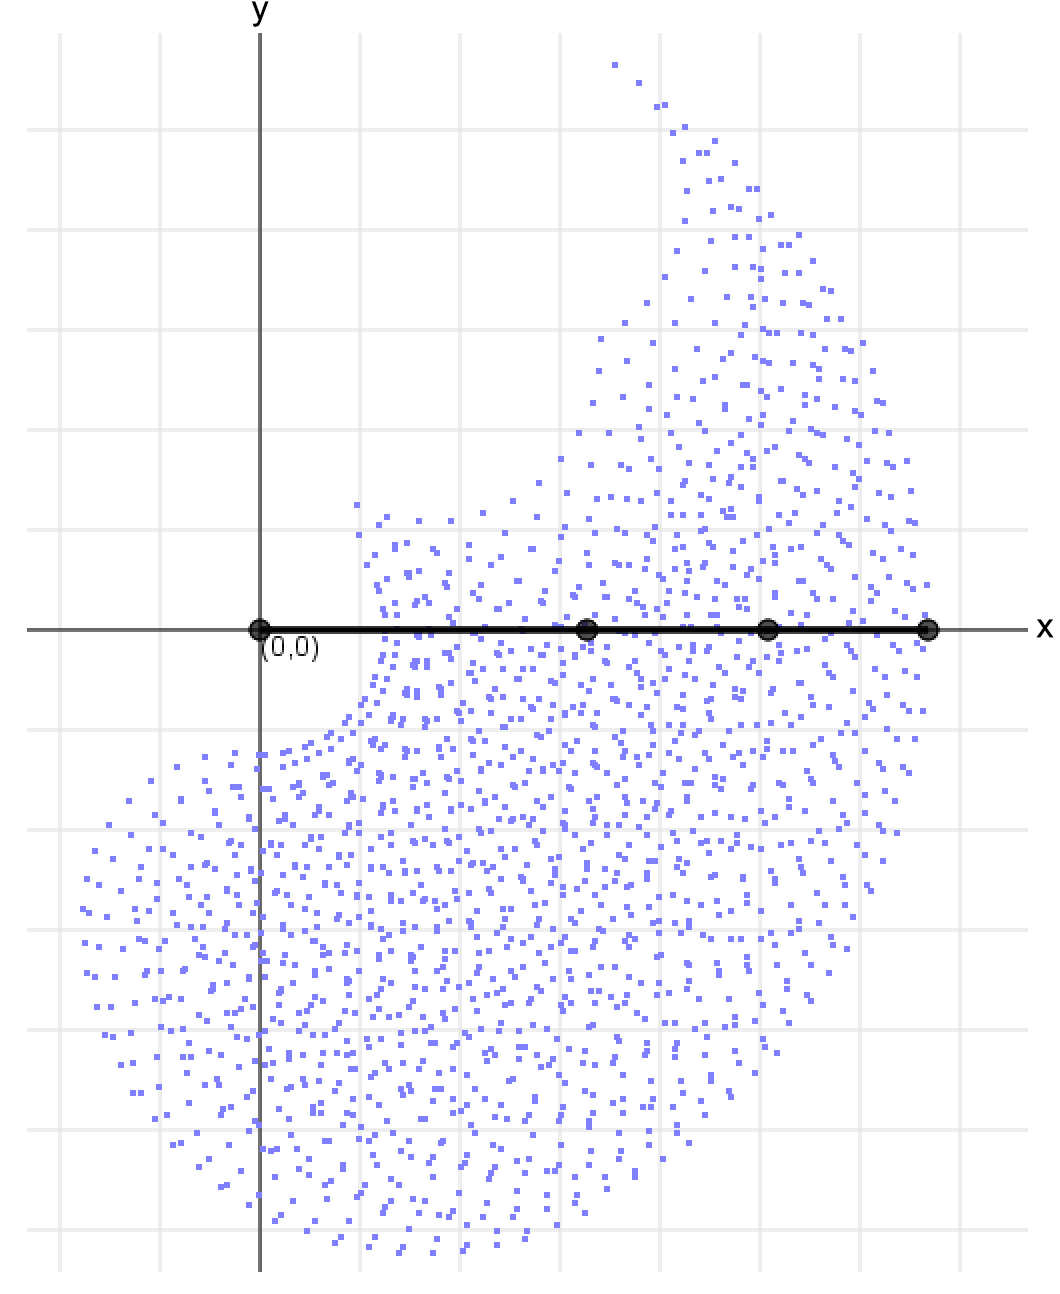
\includegraphics[scale=0.17]{reachable1.png}
\caption{Reachable positions are marked in light blue.}
\end{figure}

\newpage

\subsection{Forward kinematics with joint constraint}

Upon introducing the fixed ratio of \(\theta_3 = 2\frac{\theta_2}{3}\) the variables \textit{q} and transformation matrix \(T_3^2\) and \(T_3^0\) change.\\ 
\(T_3^2 = \begin{bmatrix}
       		\cos(2\frac{\theta_2}{3}) & -\sin(2\frac{\theta_2}{3}) & 0 & DP\cos(2\frac{\theta_2}{3}) \\[0.3em]
       		\sin(2\frac{\theta_2}{3}) & \cos(2\frac{\theta_2}{3}) & 0 & DP\sin(2\frac{\theta_2}{3}) \\[0.3em]
       		0 & 0 & 1 & 0 \\[0.3em]
       		0 & 0 & 0 & 1 \\[0.3em]
     \end{bmatrix}     
     \)\\
\begin{figure}[h!]
\(T_3^0 = \begin{bsmallmatrix}
       		\cos(\theta_1+\theta_2+2\frac{\theta_2}{3}) & -\sin(\theta_1+\theta_2+2\frac{\theta_2}{3}) & 0 & PP\cos(\theta_1) + IP\cos(\theta_1 + \theta_2) + DP\cos(\theta_1 + \theta_2 +2\frac{\theta_2}{3}) \\
       		\sin(\theta_1+\theta_2+2\frac{\theta_2}{3}) & \cos(\theta_1+\theta_2+2\frac{\theta_2}{3}) & 0 & PP\sin(\theta_1) + IP\sin(\theta_1 + \theta_2) + DP\sin(\theta_1 + \theta_2 +2\frac{\theta_2}{3}) \\
       		0 & 0 & 1 & 0 \\
       		0 & 0 & 0 & 1 \\
     \end{bsmallmatrix}\)
\end{figure}

Since the forward kinematics equations now only rely on two angles, the variables \textit{q} change to \(q = \begin{bmatrix}\theta_1\\\theta_2\\\end{bmatrix}\).

Experimenting with values between the angle variables' limits, an image of reachable positions was generated by the solver. It is clearly visible how adding the constraint limited the range of movement of the simulated finger.

\begin{figure}[h]
\centering
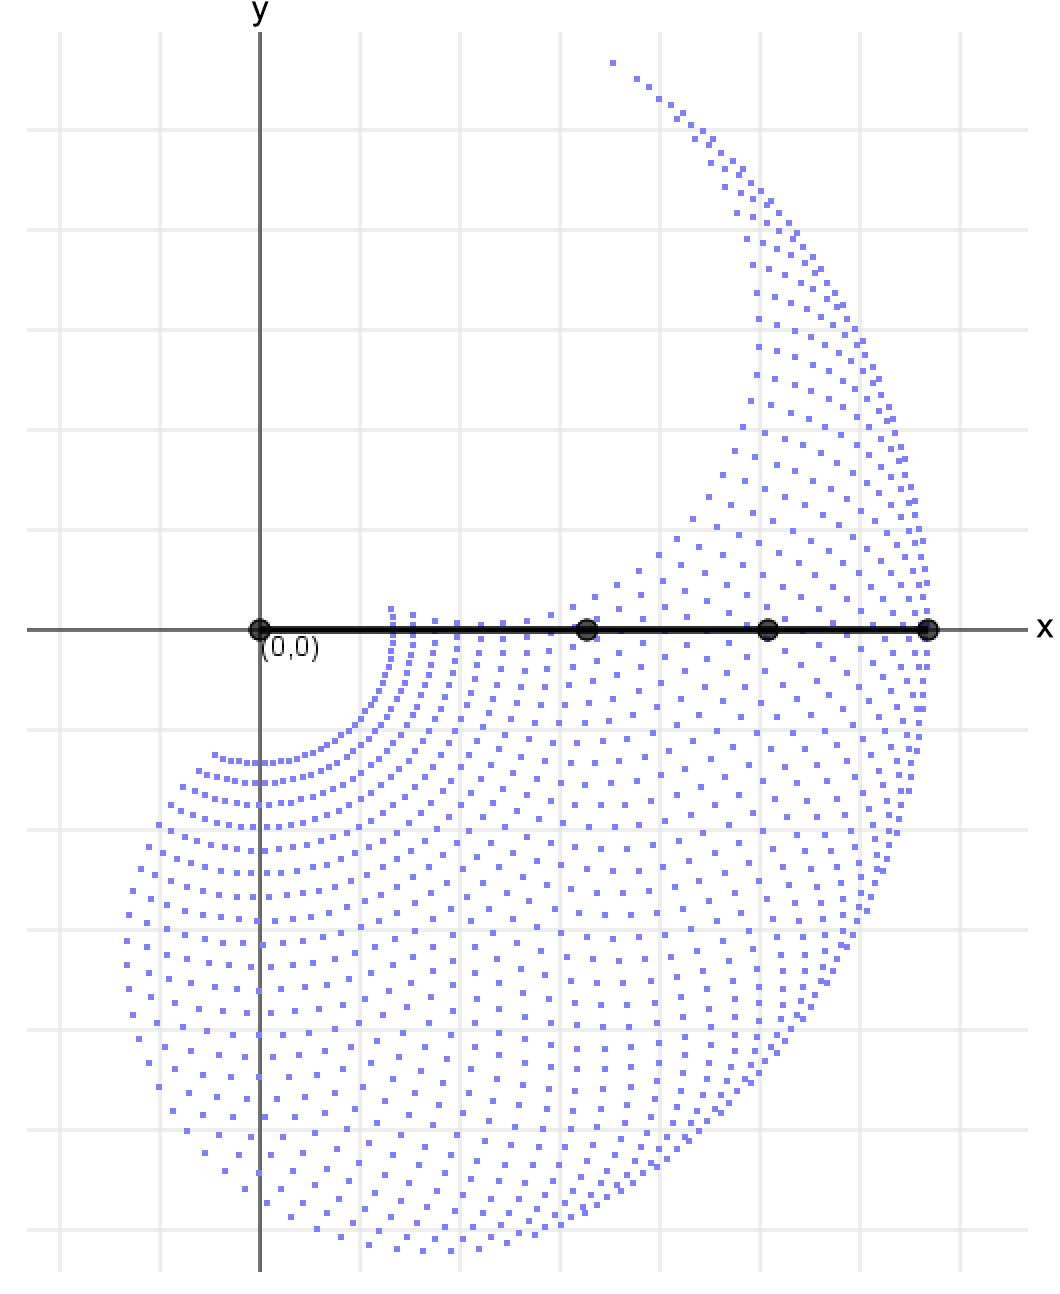
\includegraphics[scale=0.17]{reachable2.png}
\caption{Reachable positions are marked in light blue.}
\end{figure}
\newpage

\subsection{Jacobi-matrix \& inverse kinematics solver details}

Using the reworked forward kinematics transform matrices the 2x2 Jacobi-matrix \textit{J} was computed for  \(q = \begin{bmatrix}\theta_1\\\theta_2\\\end{bmatrix}\) and \(\begin{bmatrix}X\\Y\\\end{bmatrix}\), where \(X = PP\cos(\theta_1) + IP\cos(\theta_1 + \theta_2) + DP\cos(\theta_1 + \theta_2 +2\frac{\theta_2}{3})\) and \(Y = PP\sin(\theta_1) + IP\sin(\theta_1 + \theta_2) + DP\sin(\theta_1 + \theta_2 +2\frac{\theta_2}{3})\).\\

\(J= \begin{bmatrix}
\frac{\partial X}{\partial \theta_1} & \frac{\partial X}{\partial \theta_2} \\
\frac{\partial Y}{\partial \theta_1} & \frac{\partial Y}{\partial \theta_2} \
\end{bmatrix}\)

\(J =\\\\ \begin{bsmallmatrix}
-PP\sin(\theta_1) - IP\sin(\theta_1 + \theta_2) - DP\sin(\theta_1 + \theta_2 + \frac{2}{3}\theta_2)
& -IP\sin(\theta_1 + \theta_2) - \frac{1}{3}(5DP\cos(\theta_1 + \theta_2 + \frac{2}{3}theta_2))
\\PP\cos(\theta_1) + IP\cos(\theta_1 + \theta_2) + DP\cos(\theta_1 + \theta_2 + \frac{2}{3}\theta_2)
& IP\cos(\theta_1 + \theta_2) + \frac{1}{3}(5DP\cos(\theta_1 + \theta_2 + \frac{2}{3}theta_2))
\\
\end{bsmallmatrix} \)\\

An iterative, Newton-Raphson method is used in the implemented, interactive solver. The solver uses floating point values and GLM vector classes and math extensions to provide its functionality and OpenGL, SDL and SDL\_ttf to render images of the current situation to the screen (as seen earlier in the report).\\

At its very core the solver consists of three joint angles (\(\theta_1\), \(\theta_2\) and for unconstrained use \(\theta_3\)) and their constraints, three link lengths (PP, IP and DP), three  transformation matrices \(T_1^0, T_2^1\) and\( T_3^2\) and the current target position. To calculate the joint positions (including the fingertip) the forward kinematics solving algorithm is used and to find a configuration of angles which place the fingertip at a target position within the reachable area of the simulated finger the inverse kinematics solving algorithm is used.\\

The solver is (naturally) further customizable by enabling the joint constraint \(\theta_3 = 2 / \theta_2 * 3\), changing the IK-solving-algorithm's error margin \(\epsilon\) or scalar \(\alpha\). Angle arcs, circle radii and other helper lines are toggle-able. Furthermore the solver provides three demo environments for the end-user, namely a forward kinematics demo (with or without joint constraints) which can render the reachable area of the simulated finger to the screen and an inverse kinematics demo wherein the fingertip tracks the mouse position and a sliding motion of the fingertip across the surface of object \textit{O} can be initiated and rendered.\\

The forward kinematics solving algorithm uses three configuration values (the joint angles (\(\theta_1\), \(\theta_2\) and \(\theta_3\)) to update the three transformation matrices \(T_1^0, T_2^1\) and \( T_3^2\) using the Denavit-Hartenberg matrices seen earlier in the report.\\\newpage

The inverse kinematics solving algorithm guesses its first configuration values \(q_0\) and then iteratively improves on them, using the Newton-Raphson method, until it finds a suitable configuration of angles which reach the target within a specified error margin \(\epsilon\). A scalar \(\alpha\) is used for greater precision in a floating-point environment. The Jacobi-matrix is computed by filling in the matrix above. In pseudo-code:\\
\begin{algorithm}[H]
 make initial guess \(q_0\)\;
 \While{distance between target and current tip < \(\epsilon\)}{
  \If{i < maximum iterations}{
 	stop algorithm\;
  }
  solve forward kinematics for previous guess \(q_i\)\;
  calculate new tip position T\;
  calculate residue of target position and tip position\;
  calculate Jacobi-matrix J for previous guess \(q_i\)\;
  calculate pseudo inverse \(J^{+} = (J^TJ)^{-1} * J^T\)\;
  new guess \(q_{i+1} = q_{i} + \alpha * J^{+} * residue\)\;
  constrain new guess \(q_{i+1}\) to angular limits of joints\;
  i++\;
 }
 \caption{SolveIK method in pseudo-code.}
\end{algorithm}

\section{Findings of experiments}

Through slight experimentation and intuition I have found the following relations between iteration count, the initial guess and accurate solutions.

\begin{itemize}
\item{If the scalar \(\alpha\) is high, the iteration count will be low and the solution will be less accurate because of floating point inaccuracies and overshooting.}
\item{If the error margin \(\epsilon\) is high, the iteration count will be low, but the solution will be less accurate at higher error margins.}
\item{If the initial guess is close to a valid solution, the iteration count will be low.}
\end{itemize}

Using these relations several observations about initial guesses were made:

\begin{itemize}
\item{If the target \textit{T} is exactly on the edge or outside of the reachable \textit{range} (not area) our initial guess will be \(q_0 = \begin{bmatrix}\arctan(target.y / target.x)\\0\end{bmatrix}\) which handles most queried values near the edge of the reachable range well.}
\item{Other cases our initial guess will be a neutral guess in-between the limits of the angles. \(q_0 = \begin{bmatrix}
\frac{-\pi/3+\pi/3}{2}
\\
\frac{-2\pi/3}{2}
\end{bmatrix}\) which handles most queried values right of the y-axis fairly well.}
\item{Combining these cases to make the initial guess a weighted function of \(q_0 = \begin{bmatrix}\arctan(target.y / target.x)\\0\end{bmatrix}\) and \(q_0 = \begin{bmatrix}
\frac{-\pi/3+\pi/3}{2}
\\
\frac{-2\pi/3}{2}
\end{bmatrix}\) using the distance to the target as a scalar handles most queried values fairly well.}
\end{itemize}

Plotting a sliding animation on the object \textit{O} also revealed that as long as the distance between tip positions between frames is minimal, the previous frame's final guess will work quite well as the initial guess for the current frame. 

\begin{figure}[h]
\centering
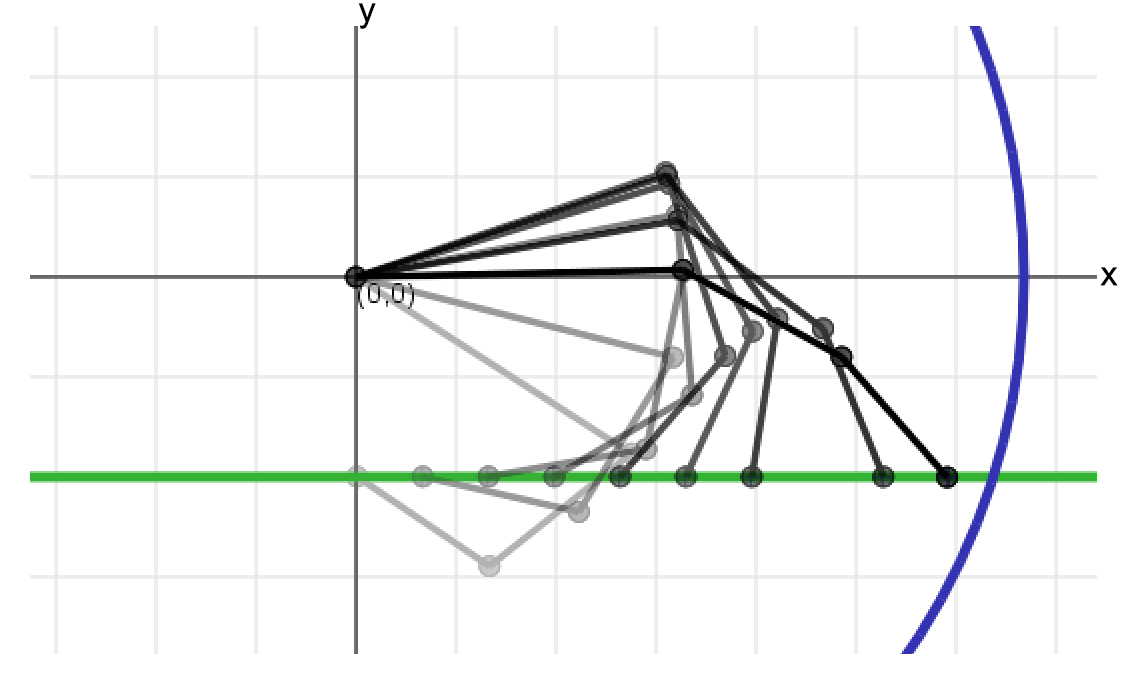
\includegraphics[scale=0.17]{animation.png}
\caption{Sliding animation on the object \textit{O}}
\end{figure}
\newpage

\end{document}